\documentclass[class = article,border = 5pt]{standalone}

\usepackage[usenames,dvipsnames]{xcolor}

\usepackage{tikz}
\usetikzlibrary{arrows, shapes, fit, backgrounds, calc}

\usepackage{amsmath, amsfonts, amsthm, amssymb}
%\usepackage{color}

\pgfdeclarelayer{background}
\pgfdeclarelayer{middleground}
\pgfsetlayers{background,middleground,main}

\setlength{\parskip}{0pt}
\setlength{\parindent}{0pt}

\begin{document}

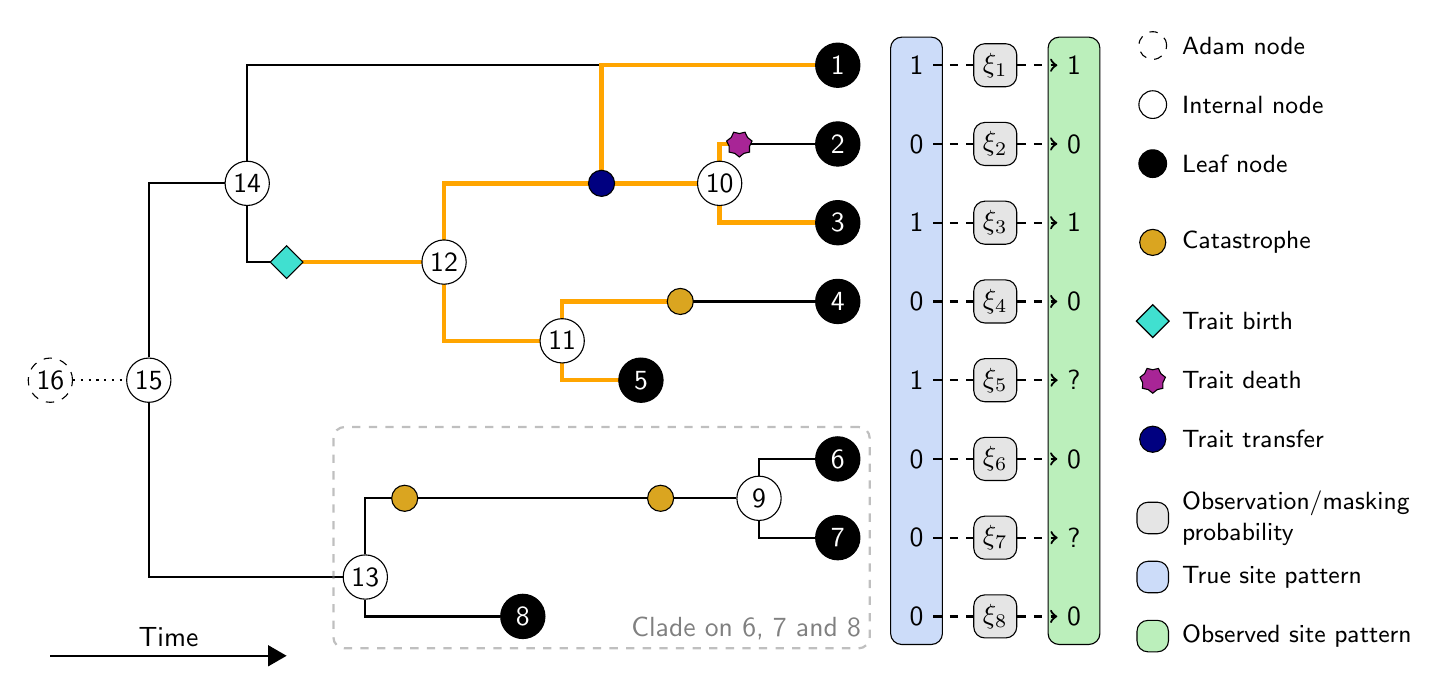
\begin{tikzpicture}

% Sans-serif text
\sffamily

% Node and arrow styles
\tikzset{nS/.style={draw, shape = circle, inner sep = 1pt, minimum width = 16pt}}
\tikzset{inS/.style={nS, fill = white}}
\tikzset{lnS/.style={nS, fill = black, text = white}}

\tikzset{pS/.style={black, thick}}
\tikzset{tS/.style={Orange, ultra thick}}

% SDLT styles
\tikzset{birS/.style={draw, shape = diamond, inner sep = 1pt, minimum size = 12pt, fill = Turquoise}}
\tikzset{deaS/.style={draw, star, star points = 7, star point ratio = 0.8, fill = Mulberry}}
\tikzset{borS/.style={draw, circle, fill = NavyBlue}}
\tikzset{catS/.style={draw, circle, fill = Goldenrod}}
\tikzset{misS/.style={draw, shape = rectangle, rounded corners, fill = black!10, align = center}}

% Clade styles
\tikzset{clS/.style={thick, shape = rectangle, rounded corners, draw opacity = 0.5, draw = black!50}}
\tikzset{clT/.style={text = black!50}}

% Label style
\tikzset{labS/.style={font = \small, align = left, anchor = west}}

% % Corners
% \node at (-0, 7.75) {};
% \node at (0, -0.75) {};

% Adam node
\node (a16) [inS, dashed] at (0, 3) {16};

% Internal nodes
\node (i15) [inS] at (1.25, 3) {15};
\node (i14) [inS] at (2.5, 5.5) {14};
\node (i13) [inS] at (4, 0.5) {13};
\node (i12) [inS] at (5, 4.5) {12};
\node (i11) [inS] at (6.5, 3.5) {11};
\node (i10) [inS] at (8.5, 5.5) {10};
\node (i9) [inS] at (9, 1.5) {9};

% Leaf nodes
\node (l1) [lnS] at (10, 7) {1};
\node (l2) [lnS] at (10, 6) {2};
\node (l3) [lnS] at (10, 5) {3};
\node (l4) [lnS] at (10, 4) {4};
\node (l5) [lnS] at (7.5, 3) {5};
\node (l6) [lnS] at (10, 2) {6};
\node (l7) [lnS] at (10, 1) {7};
\node (l8) [lnS] at (6, 0) {8};

\begin{pgfonlayer}{background}
    % Tree
    \draw[pS, dotted] (a16) -- (i15);
    \draw[pS] (i14) -| (i15) |- (i13);
    \draw[pS] (l1) -| (i14) |- (i12);
    \draw[pS] (i10) -| (i12) |- (i11);
    \draw[pS] (l2) -| (i10) |- (l3);
    \draw[pS] (l4) -| (i11) |- (l5);
    \draw[pS] (i9) -| (i13) |- (l8);
    \draw[pS] (l6) -| (i9) |- (l7);

    % Clade
    \node[clS, dashed, fit = (l6)(l7)(l8)(i13)] (s1) {};
    \node[clT, above left] at (s1.south east) {Clade on 6, 7 and 8};
\end{pgfonlayer}

% Trait birth
\node (e1) [birS] at (3, 4.5) {};

% Trait death
\node (e2a) [deaS] at (8.75, 6) {};
\node (e2b) [catS] at (8, 4) {};

% Trait borrowing
\node (e3a) [borS] at (7, 5.5) {};
\node (e3b) at (7, 7) {};

% Other catastrophes
\node (e4) [catS] at (7.75, 1.5) {};
\node (e5) [catS] at (4.5, 1.5) {};

\begin{pgfonlayer}{middleground}
    % Trait edges
    \draw[tS] (e1.center) -- (i12.center);
    \draw[tS] (e3a.center) -| (i12.center) |- (i11.center);
    \draw[tS] (e3a.center) -- (i10.center);
    \draw[tS] (e3a.center) -- (e3b.center) -- (l1.center);
    \draw[tS] (e2a.center) -| (i10.center) |- (l3.center);
    \draw[tS] (e2b.center) -| (i11.center) |- (l5.center);
\end{pgfonlayer}

% True pattern
\node (pt1) [align = center] at (11, 7) {1};
\node (pt2) [align = center] at (11, 6) {0};
\node (pt3) [align = center] at (11, 5) {1};
\node (pt4) [align = center] at (11, 4) {0};
\node (pt5) [align = center] at (11, 3) {1};
\node (pt6) [align = center] at (11, 2) {0};
\node (pt7) [align = center] at (11, 1) {0};
\node (pt8) [align = center] at (11, 0) {0};

% Observed pattern
\node (po1) [align = center] at (13, 7) {1};
\node (po2) [align = center] at (13, 6) {0};
\node (po3) [align = center] at (13, 5) {1};
\node (po4) [align = center] at (13, 4) {0};
\node (po5) [align = center] at (13, 3) {?};
\node (po6) [align = center] at (13, 2) {0};
\node (po7) [align = center] at (13, 1) {?};
\node (po8) [align = center] at (13, 0) {0};

% Masking probabilities
\node (pr1) [misS] at (12, 7) {$ \xi_{1} $};
\node (pr2) [misS] at (12, 6) {$ \xi_{2} $};
\node (pr3) [misS] at (12, 5) {$ \xi_{3} $};
\node (pr4) [misS] at (12, 4) {$ \xi_{4} $};
\node (pr5) [misS] at (12, 3) {$ \xi_{5} $};
\node (pr6) [misS] at (12, 2) {$ \xi_{6} $};
\node (pr7) [misS] at (12, 1) {$ \xi_{7} $};
\node (pr8) [misS] at (12, 0) {$ \xi_{8} $};

% Masking arrows.
\draw[pS, dashed, ->] (pt1) -- (pr1) -- (po1);
\draw[pS, dashed, ->] (pt2) -- (pr2) -- (po2);
\draw[pS, dashed, ->] (pt3) -- (pr3) -- (po3);
\draw[pS, dashed, ->] (pt4) -- (pr4) -- (po4);
\draw[pS, dashed, ->] (pt5) -- (pr5) -- (po5);
\draw[pS, dashed, ->] (pt6) -- (pr6) -- (po6);
\draw[pS, dashed, ->] (pt7) -- (pr7) -- (po7);
\draw[pS, dashed, ->] (pt8) -- (pr8) -- (po8);

% Background image
\begin{pgfonlayer}{background}

    % Site patterns
	\node (sp) [draw, shape = rectangle, rounded corners, fill = CornflowerBlue!33, fit = (pt1)(pt8)]{};
	\node (sp) [draw, shape = rectangle, rounded corners, fill = LimeGreen!33, fit = (po1)(po8)]{};

	% The arrow of time
	\draw[black, thick, ->, >= triangle 60] (0, -0.5) -- (3, -0.5);
	\node (time) [align = center, anchor = south] at (1.5, -0.5) {Time};

\end{pgfonlayer}

% Event labels
\node (al) [inS, dashed, minimum size = 10pt] at (14, 7.25) {};
\node (il) [inS, minimum size = 10pt] at (14, 6.5) {};
\node (ll) [lnS, minimum size = 10pt] at (14, 5.75) {};

\node (cl) [catS] at (14, 4.75) {};

\node (el) [birS] at (14, 3.75) {};
\node (dl) [deaS] at (14, 3) {};
\node (bl) [borS] at (14, 2.25) {};

\node (ml) [misS, minimum size = 0.4cm] at (14, 1.25) {};
\node (ptl) [draw, shape = rectangle, rounded corners, fill = CornflowerBlue!33, minimum size = 0.4cm] at (14, 0.5) {};
\node (pol) [draw, shape = rectangle, rounded corners, fill = LimeGreen!33, minimum size = 0.4cm] at (14, -0.25) {};


\node [labS] at ($ (al) + (0.25, 0) $) {Adam node};
\node [labS] at ($ (il) + (0.25, 0) $) {Internal node};
\node [labS] at ($ (ll) + (0.25, 0) $) {Leaf node};

\node [labS] at ($ (cl) + (0.25, 0) $) {Catastrophe};

\node [labS] at ($ (el) + (0.25, 0) $) {Trait birth};
\node [labS] at ($ (dl) + (0.25, 0) $) {Trait death};
\node [labS] at ($ (bl) + (0.25, 0) $) {Trait transfer};

\node [labS] at ($ (ml) + (0.25, 0) $) {Observation/masking \\ probability};
\node [labS] at ($ (ptl) + (0.25, 0) $) {True site pattern};
\node [labS] at ($ (pol) + (0.25, 0) $) {Observed site pattern};

\end{tikzpicture}

\end{document}
